\begin{blocksection}
As opposed to the TLB architecture described above, let us consider a tagged TLB. In a tagged TLB, each entry additionally contains the Address Space ID (ASID), which uniquely identifies the virtual address space of each process. A tagged TLB entry is shown below.

Tagged TLB Entry\\
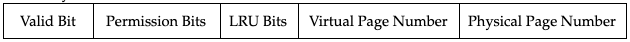
\includegraphics[width=\textwidth]{virtualmemory/taggedtlbentry}

On a lookup, we consider a hit to be if the (VPN, ASID) pair is present in the tagged TLB. This redesign allows us to keep entries in the TLB even if they are not a part of the process running on the CPU, so we do not have to flush the TLB when switching between processes. 

Consider that we are using a tagged TLB and running the code in the manner described above.

\begin{parts}
\part What is the hit rate for the tagged TLB assuming it again starts out cold? You may make the same assumptions about the variables i, j, x and ignore the effects of fetching instructions.

\begin{solution}[0.5in]
15/16. We first access a[0] , which brings in page 0 of the array for process 0. 
The first access is a miss, but the following access of a[64] is a hit because the mapping is in the TLB. 
When we switch to process 1, we access array b twice. These accesses, however, will be in the same page because they lie within a 1 KiB range and the start address of b is page­ aligned. 
Thus, we will miss the first time and hit on the second. When we switch back to process 0, the entry is already there (we don’t flush anymore) so we get 2 hits. 
Going back to process 1 will give us the same result. The next miss will occur when we get to the next page, which occurs after 4 iterations because each iteration moves 1 KiB. 
As there are 4 accesses per iteration, we have 15 hits for every 16 accesses (per process). Thus, in total, we have a hit rate of 15/16.
\end{solution}

\part What is the smallest number of entries the TLB can have to still have the hit rate found in part 4?

\begin{solution}[0.5in]
2 Entries. We need to maintain the mapping for each processes.
\end{solution}

\end{parts}

\end{blocksection}